% THIS IS SIGPROC-SP.TEX - VERSION 3.1
% WORKS WITH V3.2SP OF ACM_PROC_ARTICLE-SP.CLS
% APRIL 2009
%
% It is an example file showing how to use the 'acm_proc_article-sp.cls' V3.2SP
% LaTeX2e document class file for Conference Proceedings submissions.
% ----------------------------------------------------------------------------------------------------------------
% This .tex file (and associated .cls V3.2SP) *DOES NOT* produce:
%       1) The Permission Statement
%       2) The Conference (location) Info information
%       3) The Copyright Line with ACM data
%       4) Page numbering
% ---------------------------------------------------------------------------------------------------------------
% It is an example which *does* use the .bib file (from which the .bbl file
% is produced).
% REMEMBER HOWEVER: After having produced the .bbl file,
% and prior to final submission,
% you need to 'insert'  your .bbl file into your source .tex file so as to provide
% ONE 'self-contained' source file.
%
% Questions regarding SIGS should be sent to
% Adrienne Griscti ---> griscti@acm.org
%
% Questions/suggestions regarding the guidelines, .tex and .cls files, etc. to
% Gerald Murray ---> murray@hq.acm.org
%
% For tracking purposes - this is V3.1SP - APRIL 2009

\documentclass{acm_proc_article-sp}
\usepackage{multirow} 
\usepackage{array}
\usepackage{url}

\begin{document}

\title{MapReduce Based Resource Discovery and Monitoring System Using Self-Organizing Multicast Tree}
%
% You need the command \numberofauthors to handle the 'placement
% and alignment' of the authors beneath the title.
%
% For aesthetic reasons, we recommend 'three authors at a time'
% i.e. three 'name/affiliation blocks' be placed beneath the title.
%
% NOTE: You are NOT restricted in how many 'rows' of
% "name/affiliations" may appear. We just ask that you restrict
% the number of 'columns' to three.
%
% Because of the available 'opening page real-estate'
% we ask you to refrain from putting more than six authors
% (two rows with three columns) beneath the article title.
% More than six makes the first-page appear very cluttered indeed.
%
% Use the \alignauthor commands to handle the names
% and affiliations for an 'aesthetic maximum' of six authors.
% Add names, affiliations, addresses for
% the seventh etc. author(s) as the argument for the
% \additionalauthors command.
% These 'additional authors' will be output/set for you
% without further effort on your part as the last section in
% the body of your article BEFORE References or any Appendices.

\numberofauthors{3} %  in this sample file, there are a *total*
% of EIGHT authors. SIX appear on the 'first-page' (for formatting
% reasons) and the remaining two appear in the \additionalauthors section.
%
\author{
% You can go ahead and credit any number of authors here,
% e.g. one 'row of three' or two rows (consisting of one row of three
% and a second row of one, two or three).
%
% The command \alignauthor (no curly braces needed) should
% precede each author name, affiliation/snail-mail address and
% e-mail address. Additionally, tag each line of
% affiliation/address with \affaddr, and tag the
% e-mail address with \email.
%
% 1st. author
\alignauthor
Ben Trovato\\
       \affaddr{Institute for Clarity in Documentation}\\
       \affaddr{1932 Wallamaloo Lane}\\
       \affaddr{Wallamaloo, New Zealand}\\
       \email{trovato@corporation.com}
% 2nd. author
\alignauthor
G.K.M. Tobin\\
       \affaddr{Institute for Clarity in Documentation}\\
       \affaddr{P.O. Box 1212}\\
       \affaddr{Dublin, Ohio 43017-6221}\\
       \email{webmaster@m.com}
\alignauthor
G.K.M. Tobin\\
       \affaddr{Institute for Clarity in Documentation}\\
       \affaddr{P.O. Box 1212}\\
       \affaddr{Dublin, Ohio 43017-6221}\\
       \email{webmaster@m.com}
}
\maketitle
\begin{abstract}
Resource monitoring and discovery are important processes for building a large computing cluster.
This paper presents a MapReduce based resource query method, which runs on top of a legacy Peer To Peer(P2P) network.
A self-organizing boundedbroadcast method allows our system to query the entire network efficiently with the latency cost of $O(log^2(Number\ of\ Nodes))$.
By using the concept of Map and Reduce functional programming model, our query system performs a matchmaking in each node with the local resource information,
and the matching result is summarized and aggregated at each parent node in the boundedbroadcast tree.
Analysis and simulation result prove that our system is scalable with respect to the increased number of nodes, and the performance comparison with Sword, a DHT based resource query algorithm,
shows that our system imposes less system overhead when the number of resource information increases while providing more accurate matching result.
Our MapReduce based query system is currently deployed on the PlanetLab while using Brunet P2P network. To our best knowledge, our system is the first real-world MapReduce application that runs on top of a P2P network.
\end{abstract}

% A category with the (minimum) three required fields
\category{H.4}{Information Systems Applications}{Miscellaneous}
%A category including the fourth, optional field follows...
\category{D.2.8}{Software Engineering}{Metrics}[complexity measures, performance measures]

\terms{Delphi theory}

\keywords{ACM proceedings} % NOT required for Proceedings

\section{Introduction}
The growth of computing power in workstations and personal computers attracts substantial interest in computational clusters\cite{bonic}\cite{condor}\cite{setiathome}.
They enable sharing cpu power, storage capacity, and applications among the computers inside a cluster. These computing devices span in local, regional, or wide area network.
In order to organize and handle those widely distributed computational resources efficiently, distributed system platforms such as Condor\cite{condor}, Bonic\cite{bonic}, and SETI@Home\cite{setiathome} are proposed, 
and become a popular environment for deploying a distributed system.
After deploying such services, lots of management issues still remain. The management service should be able to distribute computation jobs evenly among cluster nodes.\footnote{In the context, node, peer, and machine will be used interchangeable}
The cluster should be scalable in case of new node join. It also has to be fault tolerant in the presence of abnormal behavior of a node or churn. 
Security issues should be addressed to prevent malicious nodes from ruining clusters.
A management system also has to support a method for monitoring nodes or locating resources in order to provide an appropriate and efficient usage of the resources or services in the cluster.
In the context of cluster's scalability, self-organizing, and fault-tolerance, a P2P network\cite{chord}\cite{pastry}\cite{can}\cite{bamboo} would be a good solution for managing node join and departure in the cluster. 
With respect to locating resources in a P2P network, a centralized indexing server might be a possible solution. 
For a node to locate resources in the network, querying to the centralized indexing server is sufficient. However, this approach is not scalable in case a huge number of nodes exist in the network.
The centralized indexing server is also a single point of failure. To overcome these limitations, Distributed Hash Table(DHT) is proposed and popularly used.
In a structured P2P network, the DHT provides a scalable lookup method in a guaranteed number of routing hops. 
However, it does not support detecting multiple hashed keys at once or matching based on a hashed value, because original DHT lookup method is based on matching a single hashed key.
To overcome the limitation of a DHT, Sword\cite{sword}, Kim et. al\cite{can_query}, and Mercury\cite{mercury} added small modifications to the original DHT to support multiple attributes query algorithm.
However, those methods impose lots of network traffic for a resource information update when the number of resource information gets bigger. 
In addition, the retrieved resource information is not always up-to-date due to the characteristics of DHT entry update period.
For the purpose of overcoming those limitations, this paper presents a distributed, decentralized, and self-organizing query method system on top of a P2P network. 
This method uses boundedbroadcast, which will be discussed in section 2.1, in order to disseminate a query to the desired region.
When a node receives a query, each node checks matchmaking based on its local information, and returns the matchmaking result to the query initiating node.
To process a query and aggregate replies from each node efficiently, we use the Map and Reduce functional programming abstraction model.
We deployed our MapReduce based query system on the PlanetLab\cite{planetlab} with legacy P2P network, Brunet\cite{brunet} in order to address the feasibility and efficiency of our approach. 
We compared the performance of our query system with SWORD\cite{sword} analytically and through simulation.
Our query system's characteristics and contributions are the following:
\begin{enumerate}
\setlength{\itemsep}{0pt}
\setlength{\parskip}{0pt}
\item It imposes no resource information update traffic, because each query is resolved using the a node's local resource information.
\item Each node processes matchmaking based on the local machine's information, so the query response is always up-to-date.
\item Boundedbroadcast provides an efficient way to disseminate a query to the entire network by using a self-organizing tree.
\item By using the Map and Reduce functional programming model, our system modularizes query and response processing cleanly.
\item Based on our knowledge and survey, MapReduce based query system is the first real-world MapReduce application deployed on a legacy P2P network.
\end{enumerate}
The rest of this paper is organized as follows. 
Section 2 discusses MapReduce based query system architecture. 
Section 3 evaluates our query system model and compares the performance with that of SWORD by simulation and analysis. Section 4 discusses related work.
Section 5 summarizes and concludes this paper.

\section{System architecture}
In this section, we describe the overall architecture of the MapReduce based query system and boundedbroadcast method. 
We will also discuss how we use Map and Reduce function to handle a query and response processing.
\subsection{Boundedbroadcast}
The purpose of boundedbroadcast\cite{deetoo} is to distribute a message to a sub-region of a P2P network by using a self-organizing tree.
A node which is responsible for disseminating a message redistributes the message to its neighbor nodes which reside inside its allocated sub-region while allocating new sub-regions to the neighbor nodes appropriately.
Those nodes which receive the message redistribute the message using same manner.

Boundedbroadcast is currently implemented on top of Brunet\cite{brunet}, which implements a 1-d Kleinberg small-world network.
Each Brunet node maintains two kinds of neighbor connection: an adjacent node connection and a distant node connection.
To broadcast a message over the sub-region[A,L] in Figure 1(a), a message initiator inserts a broadcast command to node A with sub-region information, [A,L]. 
Node A recognizes node B and P as its adjacent neighbor nodes, and  E, K, L, and M as its distant or short-cut connection neighbors.
Based on the node A's connection table, node A disseminates broadcast messages only to its neighbors, by specifying broadcast range as [B~E), [E~K), [K~L), [L] to node B, E, K, and L, respectively.
After receiving the message, node B, E, K, and L broadcast the message only to its neighbor nodes inside the specified sub-region recursively. 
After disseminating the broadcast message until the leaf node, a graph like Figure 1(b) is formed.

If the broadcast message initiating node does not lie in the boundedbroadcast region, the broadcast message is first routed to a center node inside the boundedbroadcast region using greedy routing.
Boundedbroadcasting method is responsible for distributing queries to nodes in the P2P pool and dealing with lagging nodes whose response time takes longer than the others. 
The latency cost of boundedbroadcast is  $O(\log^2(N))$ \cite{deetoo}, which is larger than a DHT system ($O(\log(N))$)\cite{chord}, but smaller than a naive flooding based broadcast method($O(N)$).
\begin{figure}
\centering
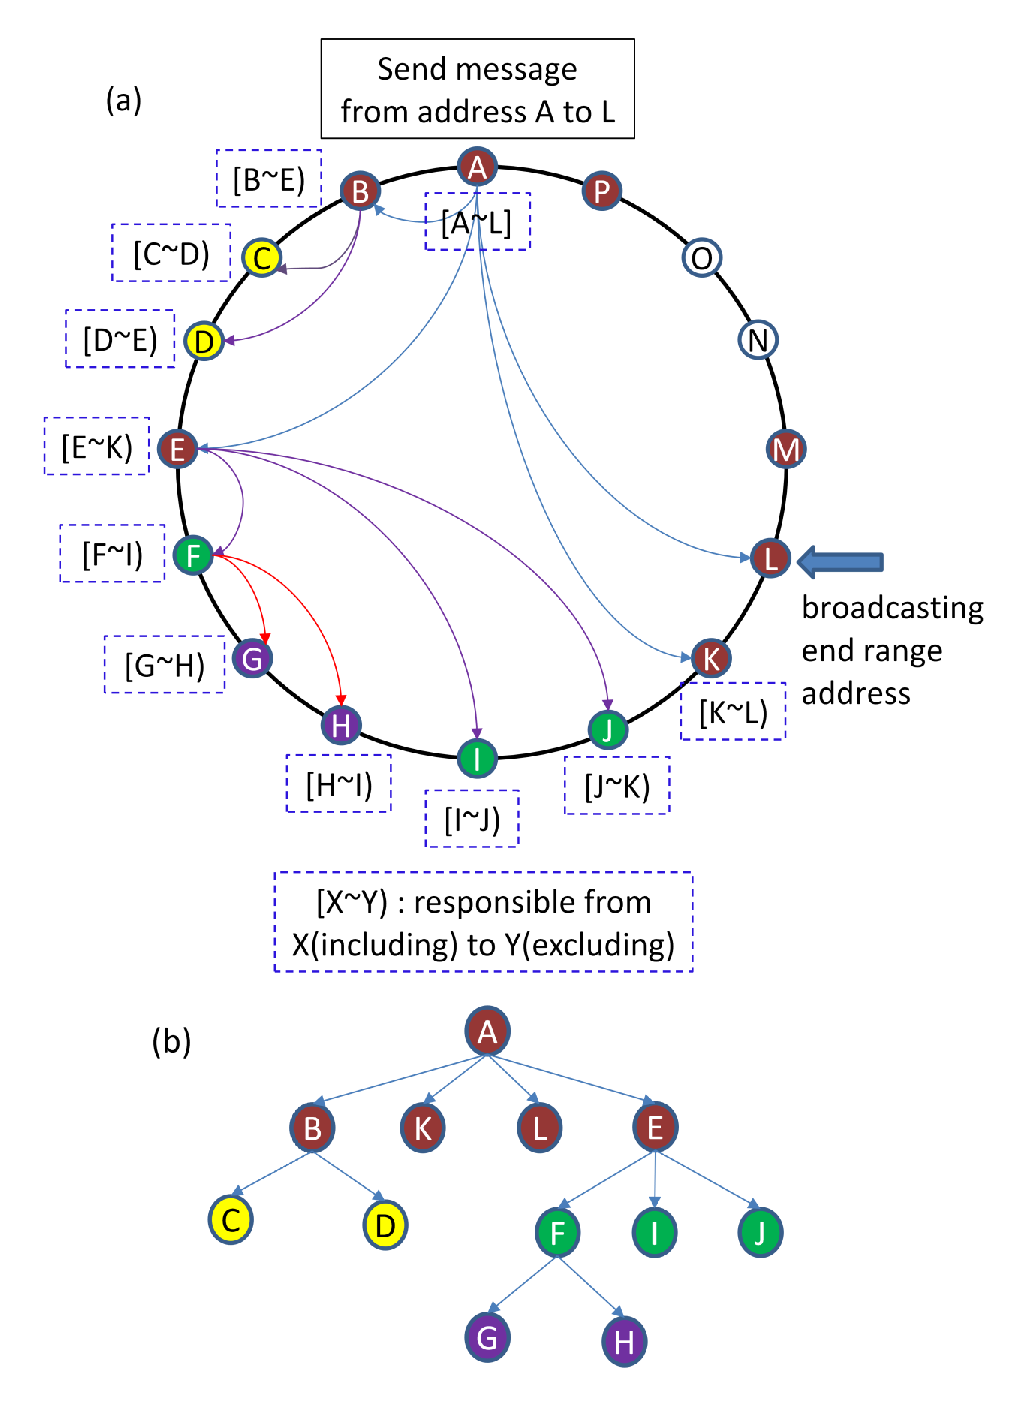
\epsfig{file=bb1.eps, width=3.4in}
\caption{Boundedbroadcasting message propagation}
\end{figure}

\subsection{MapReduce}
Map and reduce function are used in the Lisp programming language and many other functional programming languages. 
Based on the concept of map and reduce function of the functional programming model, Google proposed a software framework to parallelize large dataset computations efficiently\cite{google_mapreduce}.
Map function usually works on (Key/Value) pairs to create intermediate (Key/Value) results. 
Result functions work on intermediate (Key/Value) results while aggregating intermediate values associated with the same intermediate keys.
The MapReduce framework supports distributing map and reduce tasks among nodes in a cluster to enable parallel processing, dividing input files into multiple chunks,
and rescheduling a late processing job. Thus users do not have to take care of detailed management issues for distributed parallel job execution. Instead, the users have to define the 
map and reduce functions associated with their needs.
The open group also provides MapReduce function called Hadoop MapReduce\cite{hadoop}

In our MapReduce based query system, we defined the Map function as checking requirement matching and calculating rank value. The Reduce function is defined as 
aggregating and ordering the Map result based on the matching result and rank value. We will look into MapReduce based query system's Map and Reduce functions in detail in the section 2.C. 
In section 2.D, we will discuss the differences between Google MapReduce and our MapReduce based query system.

\subsection{MapReduce Based Query System Architecture}
MapReduce based query system is divided into 5 modules. They are P2P network module, MapReduce core , Map and Reduce function, local resource information monitor, and matchmaking module.
We will discuss those 5 modules thoroughly in the following sections and combine them together for the entire query system.
\subsubsection{P2P Network Module}
Underlying P2P network module is responsible for handling new node join and departure, connection managements with neighbor nodes, and routing messages. 
The current version of MapReduce query system is developed on top of Brunet\cite{brunet}, which implemented the 1-D Kleignberg's small world network\cite{small_world_network}.
However, our system can be deployed on the other P2P platforms, such as Chord\cite{chord}, CAN\cite{can}, or Pastry\cite{pastry} if those platforms
provide an efficient broadcasting method, such as boundedbroadcast. 
\subsubsection{MapReduce Core Module}
The MapReduce core module takes responsibility for distributing Map and Reduce functions using boundedbroadcast, discussed in section 2.1. 
When a user initiates a MapReduce task, the request is conveyed to the MapReduce core module through underlying P2P network's Remote Procedure Call(RPC) module. 
MapReduce core module checks the Map argument, the Reduce argument, and the broadcast sub-region argument. 
The Map and Reduce argument will be passed to the Map and Reduce function, respectively. 
The broadcast sub-region argument describes a boundedbroadcast region, where the node is responsible for. 
The MapReduce core module disseminates the task to nodes which reside under its responsible region after manipulating broadcast sub-region argument appropriately.
\subsubsection{Map and Reduce Function Module}
\begin{figure}
\centering
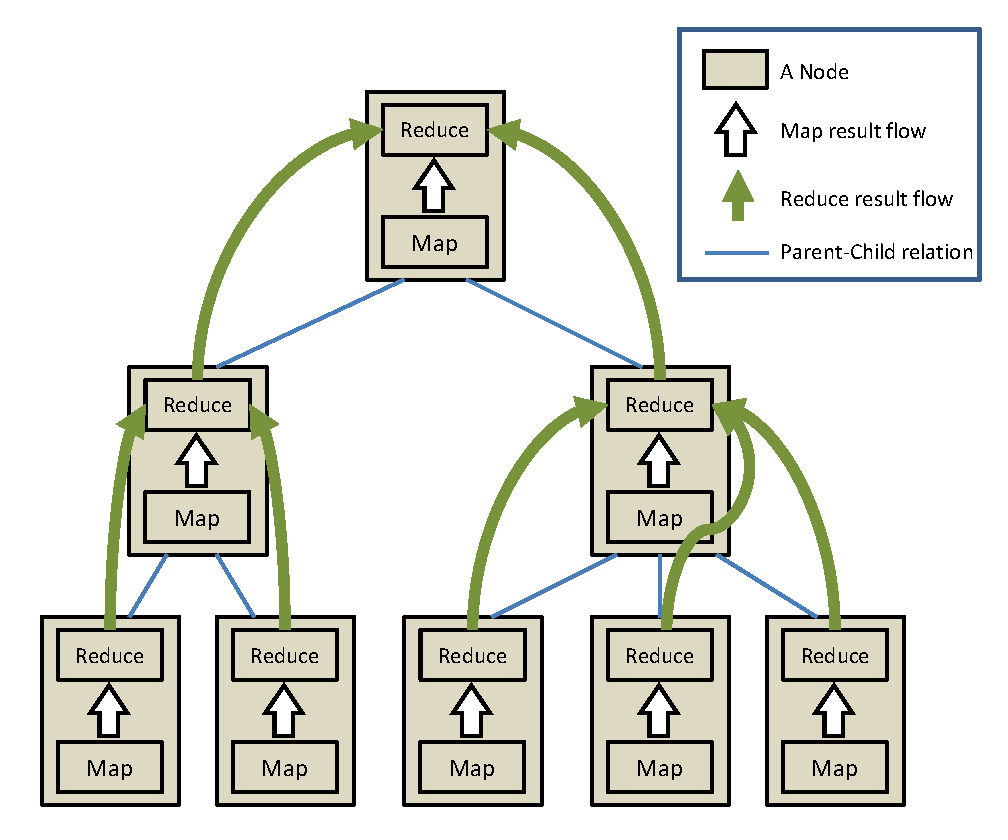
\epsfig{file=mr_struct.eps, width=3.4in}
\caption{Map and Reduce result flow}
\end{figure}
Similar to the Google MapReduce, a user has to define its own Map and Reduce functions associated with his needs. 
After a node processes the Map task, the node returns the result to the Reduce function of itself.
The Reduce function aggregates its own Map result and child nodes' Reduce results. 
After completing the Reduce function, the node returns the result to the parent node's reduce function.
We visualize the dataflow between the Map and Reduce functions in the Figure 2.
For the resource discovering purpose, the Map and Reduce functions are defined as follows:

\textbf{Map function}: In a Map function, a resource requirement and a rank criteria are delivered as a Map argument .
\begin{flushleft}Requirement=(other.Memory>2048) \&\& ((other.KeyboardIdle>300) || LoadAvg<0.3))\ \ \ \ \ \ \ \ (1)\end{flushleft}
\begin{flushleft}Rank=(other.Memory)+(other.KeyboardIdle*10)\ \ \ (2)\end{flushleft}
(1) describes the resource requirement. It means that the target resource's memory has to be bigger than 2GB and the keyboard idle time is more than 300 seconds or the average load is less than 0.3.
When a node receives a resource matching request, it first checks whether it satisfies the requirement or not. If it does, it calculates the rank value whose purpose is to order the requirement satisfying nodes.
(2) shows the rank criteria. Every node which satisfies the requirement calculates its rank value using given rank criteria. In this example, the rank value is calculated as Memory size + Keyboard idle time*10.
As we can see from this example, a user can easily specify its requirement and the requirement satisfying nodes ordering method arbitrary.
For a matchmaking purpose, we use the Condor ClassAd\cite{classad} to exploit its regular expression matching and arbitrary matching support.
Using Condor ClassAd allows us for ordering the requirement satisfying nodes more flexible than Kim et. al\cite{can_query}, which supports only the static ordering method(i.e., based on average queue size and cpu speed)

\textbf{Reduce function}: In the Reduce function, the number of desired nodes and a rank ordering method are delivered as an input argument.
Assuming that a node sends a MapReduce task to $n$ nodes using boundedbroadcast, \begin{math}n\end{math} reduce results will be returned from the child nodes, 
and one Map result will be returned from itself. The Reduce function will aggregate and summarize those results based on the number of desired nodes, an ordering method, and rank values. 
Number of desired nodes specifies how many nodes the user wants to find in the pool, and an ordering method specifies rank value alignment method. 
If the number of desired nodes is $k$, and the ordering method is \textit{ascending}, the rank value is aligned in the ascending order, and top k rank value nodes are returned from the Reduce task.

\subsubsection{Local Resource Information Monitor Module}
There are several ways to gather resource information. The naive way would be using \textit{/proc} file system on the Linux machine. 
By using the \textit{proc} file system, we can get the kernel information, process information, cpu information, memory information, and etc. 
Because a lot of linux commands(ps, top, pstree, and etc) rely on the information provided by the \textit{/proc} file system,  
the programmer can choose either way(/proc file system or linux commands), which is convenient. 
Though this method is simple and easy to access, it provides only limited amounts of information. In addition, this information is not accessible on operating systems other than Linux.
We can use the Comon\cite{comon}, which  is a PlanetLab\cite{planetlab} node monitoring system, as resource information gathering purpose. The system not only passively gathers the resource information
provided by an operating system, but also actively aggregates and summarizes resource information metrics useful for a system administrator and users. 
It also supports a dynamic query language to enable users to monitor PlanetLab deployed applications.
Due to its initial development purpose, it is currently deployed only on the Planetlab. The Comon developer does not provide a way to run the system in a standalone mode, which would be independent of the PlanetLab. 
The Condor\cite{condor} uses a condor\_startd daemon to monitor and gather resource information. 
This daemon periodically sends a machine's Classified Advertisements(ClassAd)\cite{classad} to a condor\_collector daemon. 
The machine's ClassAd is used to evaluate matchmaking by a condor\_negotiator. 
As of Jan. 2010, the Condor 7.5.0 system is released for various Linux systems, Windows, and Mac. The system allows running each condor daemon in a standalone mode without
installing entire Condor pool. It provides summarized metrics, such as load average and total idle time, as well as basic information provided by an operating system.
\subsubsection{Matchmaking Module}
We used the condor ClassAd\cite{classad} to check whether an user's requirement satisfies the resource's capacity or not. 
With a connection to the condor\_startd daemon, the ClassAd provides a clean interface to interact with the resource information provided by condor\_startd. 
After getting the local resource information through the condor\_startd as an XML file, a ClassAd library converts the XML file into a ClassAd object, which is suitable for a matching purpose.
Two ClassAd objects(i.e., resource information ClassAd and job requirement ClassAd) match if both ClassAds contain the requirement field, and the requirement value evaluates to \textit{true} to the other ClassAd. 
For example, \textit{requirement=other.NumberOfCPU>2} will match with a resource which has more than two processors.
As of January 2010, C++ and Java version of ClassAd source codes are provided, and we use the Java ClassAd library for matchmaking purpose. 
Because we use the ClassAd library intact, our query system follows most of the ClassAd library characteristics.(e.g., supporting range query, regular expression match, and etc.)
\begin{figure}
\centering
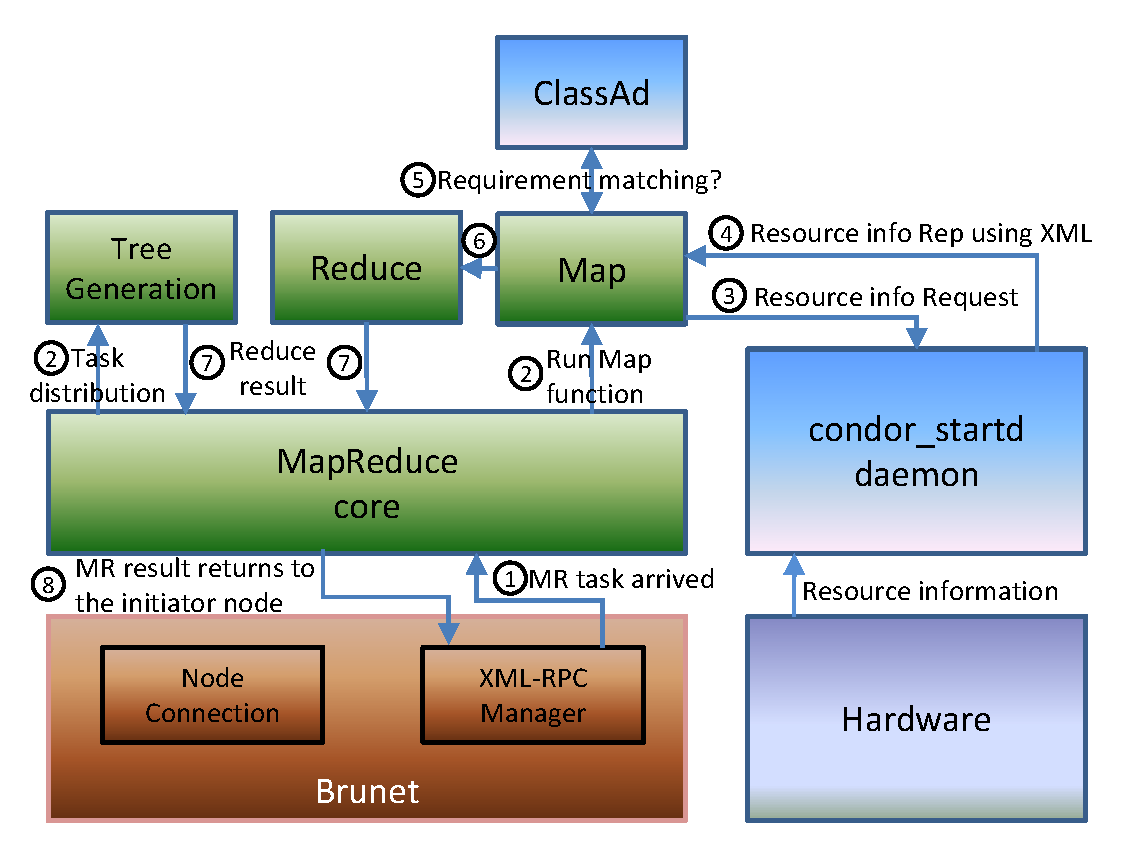
\epsfig{file=structure.eps, width=3.5in}
\caption{MapReduce resource discovery system architecture}
\end{figure}

Using the five modules described from the section 2.A to 2.E, Figure 3 architecture is formed. MapReduce based resource discovery processing step is as follow:
\begin{enumerate}
\setlength{\itemsep}{0pt}
\setlength{\parskip}{0pt}
\item When a MapReduce task arrives to a node, it is delivered to the MapReduce core module first.
\item The MapReduce core module redistributes the task to nodes which reside inside the node's allocated sub-region and waits the results from the child nodes. MapReduce core also runs a local Map function.
\item The Map function requests local resource information to condor\_startd daemon.
\item The condor\_startd returns the up-to-date resource information expressed as an XML.
\item The Map function converts the returned XML-resource information to a ClassAd object and checks requirement matching using the ClassAd.
\item The local resource matching result is returned to the local node's Reduce function.
\item The local node's reduce result and child nodes' Reduce results are returned to the MapReduce core, and the result is aggregated.
\item The MapReduce core module returns the aggregated Reduce result to the MapReduce task initiating node.
\end{enumerate}

\subsection{Differences Between Google MapReduce and MapReduce Based Query System}
In this section, we are going to highlight the differences between the Google MapReduce and our MapReduce based query system.
\begin{description}
\item[Goal]The goal of the Google MapReduce is sharing computing power for processing large dataset.\cite{google_mapreduce}. Due to its large dataset transfer, it is appropriate for using in a LAN environment.
Our MapReduce based query system, on the other hand, targets for monitoring and querying a cluster's nodes in a WAN environment.
\item[Central Manager]Google MapReduce runs one central manager which deals with assigning map and reduce task, and reallocating a failing worker node's job.
Due to the central manager node's job assigning task and periodical worker nodes' health check, the central manager can be a bottleneck or a hot-spot node. 
On the contrary, our MapReduce based query system has no centralize manager node. Instead, a self-organizing boundedbroadcast tree is responsible for committing map and reduce tasks.
\item[Handling Lagging Nodes]The Google MapReduce does not provide a method to handle lagging node, but Hadoop MapReduce does. In Hadoop, a lagging node is detected based on a progress score.
If a node's progress score is less than a threshold value, which is decided based on the average Map and Reduce task execution time, the node is marked as a straggler. The straggler node's job is reassigned by a central manager node.\cite{hadoop}
The Late scheduler\cite{late} selects a lagging node that will finish the farthest into the future. They predict the job completion time based on \textit{Remaining Job Portion / Progress Rate}, which considers both
how fast the node is processing the task and how much amounts of work remains.
Both Hadoop and Late algorithm obligate a central manager node monitoring Map and Reduce task execution nodes. 
In MapReduce based query system's case, RPC timeout will distinguish lagging nodes. If a node lingers and makes a RPC timeout, the retarding node's child nodes' results will be wasted, 
because the parent node will prune the lagging node from a boundedbroadcast tree. Handling child node's timeout gracefully and getting partial results from a lagging node are one of our future works.
\item[Network Bandwidth Usage]Based on each method's goal, the Google MapReduce consumes lots of network bandwidth, and it needs a fast data transmission for an efficient job processing. 
Oppositely, MapReduce based query system consumes small amount of network bandwidth, because the Map argument(i.e., query requirement) is usually less than several-hundred bytes, and the Reduce result is aggregated at each node in the tree.
The hierarchical information aggregation method, which applies to the Reduce result accumulation, provides scalability in a distributed information management system.\cite{astrobe} \cite{treedatamanage}
\end{description} 

\section{Evaluation}
In this section, we evaluate the MapReduce based query system in a decentralized and heterogeneous environment using an analytical method and a simulation. 
To address the feasibility of the MapReduce based query system in the real-world, we deployed the MapReduce based query system on the PlanetLab. 
To compare our MapReduce based query approach against a DHT based range query algorithm, we evaluate SWORD\cite{sword} analytically and via a simulation.
\subsection{SWORD}
The SWORD range query method shares the ultimate objective with the MapReduce based query system, whose goal is to allow end users to locate a subset of nodes which satisfy the users' requirement in a cluster.
The SWORD provides matchmaking service using a DHT system. The original DHT system works based on a <key, value> storage. 
Each key is hashed to a node id, and the appropriate node, whose node ID is the closest to the hashed key value clock-wise direction on a ring structure\cite{chord} \cite{pastry}, keeps the <key, value> pair. 
Thus, simply matching an attribute name and a value to a DHT entry's key and value cannot support a resource discovery. 
To overcome this limitation, the SWORD maps an attribute name and a value to the DHT entry key. Among $n$ bits of a DHT key size, it allocates $m$ bits as attribute index bit, where $n>m$. 
Of the remaining $n-m$ bits, $k$ bits are designated as value expression bits, and a random value is filled in the remaining $n-m-k$ bits. Figure 4 shows a mapping of a measured value to a DHT key.
The mapping is performed once per an attribute for every information update event, and the entire resource information is conveyed to the calculated DHT key as a value.
\begin{figure}
\centering
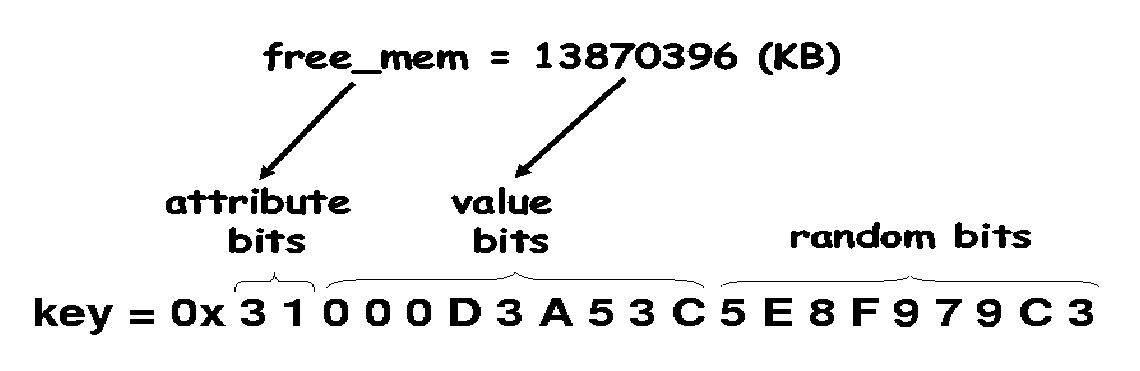
\epsfig{file=sword_key.eps, width=3.4in}
\caption{SWORD DHT key mapping}
\end{figure}
To find nodes whose free memory is between 1GB and 2GB, the SWORD first has to determine query begin address and query end address. 
To decide the query begin address, it sets the attribute bits as a pre-determined free memory attribute index, the value bits as 1GB, and the random bits as all 0x0s.
For the query end address, it also sets the attribute index bits, the value bits as 2GB, and the random bits as all 0xFs to cover all random bits value. 
If multiple attributes need to be considered, one representative attribute is selected randomly, and the query range is determined based on the requirement of the randomly selected representative attribute.
Other than a naive resource matching, the SWORD provides an \textit{optimizer} module to select optimal resources among multiple candidate nodes. 
\subsection{Performance Analysis}
In this section, we are going to compare the performance of the MapReduce based query system and SWORD analytically. 
Our analysis focuses on the Number of Visited to Complete a Query-$N_Q$, Query Latency-$L_Q$, Query Bandwidth-$B_Q$, Resource Information Update Bandwidth-$B_U$.
We express the total number of nodes in a pool as $N$, the number of published attributes as $A_N$, the size of each attribute as $A_S$, a resource information DHT update period as $U_P$, 
and the number of attribute and value indexing bits shown in the Figure.4 as $I_A$, and $I_V$, respectively. In this analysis, we assume that all nodes in a pool are evenly distributed through the all address region.

\subsubsection{Number of Visited Nodes to Complete a Query}
The MapReduce based query system visits all nodes in the pool, so the number of visited node to complete a query is $N$.
SWORD can optimize this metric by manipulating the number of bits for an attribute and a value indexing bits in Figure 4. As the number of bits for an attribute and a value indexing increases by 1 bit, 
the query region decreases in half. Thus, the number of visited nodes to complete a query is\begin{math}\frac{N}{2^{I_A+i_v}}\end{math}, where \begin{math}0<i_v<I_V\end{math}.
\begin{math}i_v\end{math} means the number of same bit value between query begin and end value. For example, if a query wants to find machines whose attribute value lies between 0x0000 and 0x00FF, \begin{math}i_v\end{math} is 8. 
\subsubsection{Latency For a Query}
The latency of a query depends on the number of visited nodes to complete a query. Because MapReduce based query system propagates queries using boundedbroadcast, the latency closely related to
the tree-depth of the boundedbroadcast. According to the DeeToo\cite{deetoo}, tree depth of a boundedbroadcast is \begin{math}O(log^2(N))\end{math}. Assuming SWORD query is propagated using boundedbroadcast,
the query latency will be  \begin{math}O(log^2(\frac{N}{2^{I_A+i_v}}))\end{math}. Otherwise, the latency of MapReduce based query system is  \begin{math}O(log^2(N))\end{math}.
\subsubsection{Bandwidth Usage For a Query}
Let's assume that a query message size is $S_Q$, and a response message size is $S_R$.
In the boundedbroadcast, a message is routed only to the 1-hop neighbors, so the query and the response message size between a parent and a child node is $S_Q+S_R$.
Thus, the bandwidth usage to complete a query is \begin{math}(N_Q-1)*(S_Q+S_R)\end{math}.
In case of the MapReduce based query system, Reduce results from child nodes are aggregated whenever a parent node processes a Reduce function, so $S_R$ of MapReduce based query system does not increase
as the Reduce results propagate through the boundedbroadcast tree.

As we can see from the above three metrics, the query performance is closely related to the \textit{Number of Visited Node to Complete a Query}. By using the boundedbroadcast, we can complete a query
at the cost of \begin{math}O(log^2(N_Q))\end{math}, which is smaller than flooding based broadcast cost(\begin{math}O(N_Q)\end{math}).
\subsubsection{Cost for Resource Information Update}
The SWORD checks a query matching at nodes which lie inside the query range. To perform the query matching at the distant nodes, resource information has to be periodically updated at the proper remote nodes.
Otherwise, MapReduce based query system does not need any resource information update, because query matching is processed using local resource information at the Map function.
In this section, we are going to analyze the SWORD's bandwidth cost to update resource information to remote nodes.
Every node has to update its resource information, whose size is $A_N*A_S$(neglecting serialization overload), $A_N$ times, because any nodes which are mapped to the hashed key has to provide query matching service. 
Because of the soft-state properties of the DHT, each entry has to be updated at least every $U_P$ seconds. All nodes($N$) in the pool will perform this update.
In addition, each DHT entry has to be routed to a proper hashed key node, which takes $O(log(N))$ hops\cite{chord}\cite{pastry} or \begin{math}O(\frac{1}{k}log^2(N))\end{math},where $k$ is number of short-cut connection\cite{brunet}.
Accordingly, the bandwidth consumption for a resource information update per one update time period is:
\begin{displaymath}N*A_N*(A_N*A_S)*(\textit{Number of Hops})\end{displaymath}
It shows that the bandwidth consumption is $O(A_N^2)$, and O(N), which is not scalable in case of increasing number of resource information attributes.
\subsubsection{Query Result Correctness}
Each resource information saved in the DHT entry is not usually up-to-date. This may not hurt the SWORD performance if the query is based on static resource information, such as operating system. 
When it comes to dynamic information, such as current cpu load or free memory size, the stale information is highly likely to be useless. 
Because a DHT entry age is dependent on the DHT entry update period, the SWORD can make the period shorter to keep the resource information fresher.
However, it will result in more frequent DHT entry update and more bandwidth consumptions.
\subsection{Simulation Results}
\begin{figure}[t]
\centering
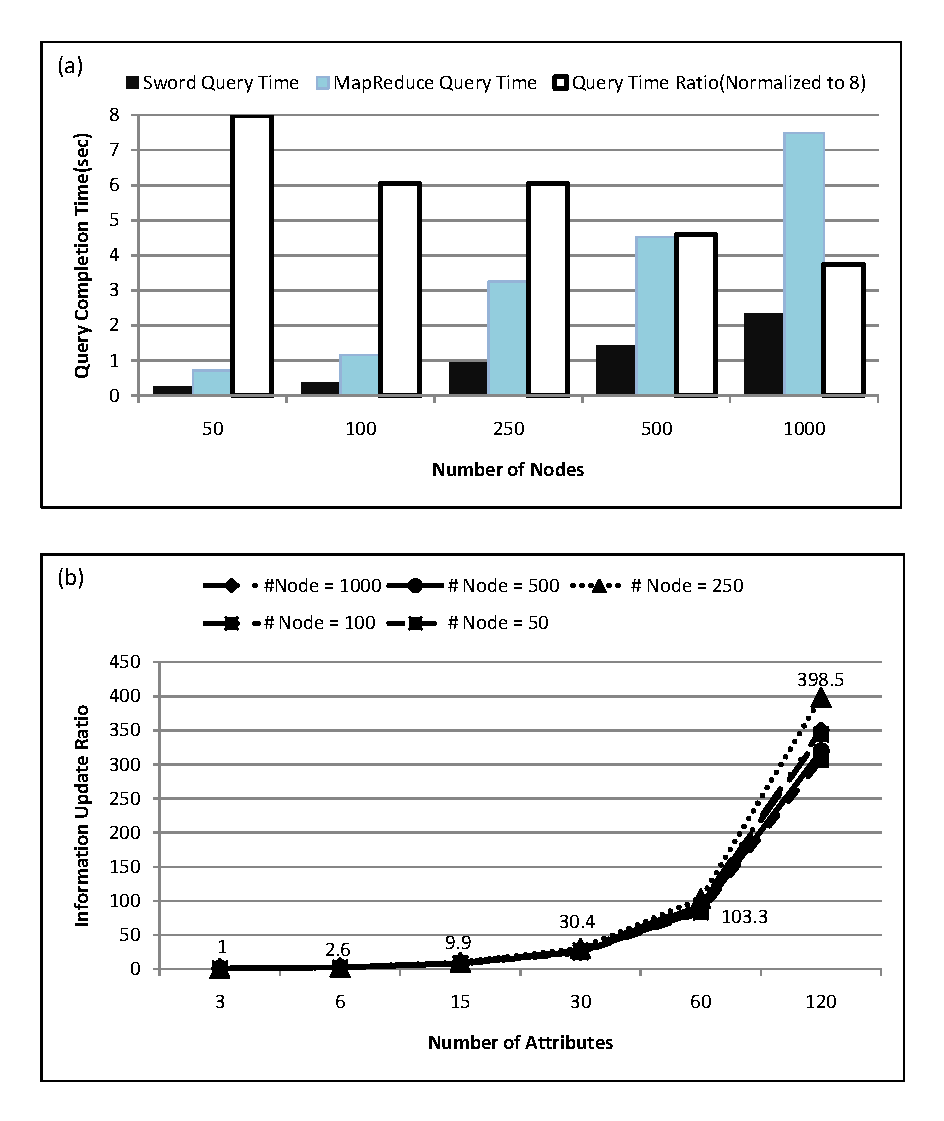
\epsfig{file=sim.eps, width=3.4in}
\caption{MapReduce based query system and SWORD simulation result (a)Query completion time. Query time ratio = (Query complete time/Number of nodes)*1.6. 
(b)SWORD resource information update size. Ratio=(BW consumption)/(BW consumption when the number of attribute is 3)}
\end{figure}
To allow complete analysis and compare the performance of MapReduce based query system and SWORD, we implemented an event-driven single-threaded simulator, which uses Brunet\cite{brunet} routing, DHT, and node management.
This simulator provides us a controlled experiment environment, and also allows us to check the correctness of our system implementation. We used MIT King data set\cite{king} to set network latency between nodes.
Using Archer\cite{archer}, we could run the simulation on a decentralized computing cluster efficiently. 
On the simulation, we ran 1-simulated hour after the P2P pool is formed to make the pool stable. After then, target operation(i.e. resource query or DHT resource information update) is initiated at each node for 2-simulated hours.
For the MapReduce based query system, each node initiates a query every 5 minutes while setting the query range as the whole network. 
In case of SWORD, we allocated 4 bits for attribute indexing, and the value field is filled with two randomly generated int or double value to specify a desired region. 
We set the Time To Live(TTL) of SWORD's DHT entry as 30 minutes, and the entry update is performed every 15 minutes.
After running 10 simulations with different parameters, we calculated the average value.
\subsubsection{Query Complete Time}
Figure 5.(a) shows query completion times. As we can see from the figure, the query time grows as the number of nodes increases. To highlight a relation between a query complete time and a number of nodes,
we added the query time ratio value. The ratio is calculated as \begin{math}\frac{Query\ Complete\ Time}{Number\ of\ Nodes}\end{math}, and multiplies a constant value to make the value fit for the graph.
The ratio value decreases as the number of node increases, so we can conclude from this pattern that the order of our query system latency is less than $O(N)$, but bigger than $O(log(N))$.
Though SWORD shows less query latency than MapReduce based query system, the actual effect of SWORD's less query region is not so remarkable. 
When we set 4 bits for the attribute indexing, the SWORD query region is about 0.3\% of the entire network. 
However, the query latency decreased only to about 30\% of entire network query latency, while the query region is decreased to 0.3\%.
It may show different latency values for the other P2P network systems, but we can conclude that the cost for querying the entire network would be small if we design the boundedbroadcasting system while considering
each P2P network's characteristics carefully, which is one of our future works.
\subsubsection{Query Bandwidth Usage}
Table. 1 shows the bandwidth consumption to complete a query. The \textit{Ratio} value is calculated as \begin{math}\frac{SWORD Bandwidth}{MapReduce bandwidth}\end{math}. The ratio value decreases as the number of nodes
increases, but it is still bigger than 0.3\%, which is the fraction of the SWORD query region to the entire network. One of the reason is multiple hops to route a message to a node which resides in the query region.
A probability to find a node in a SWORD query region will decrease when the number of node in the pool decreases, so it will take more hops to route a message to a node in the desired region. 
In our simulation, the number of node in a query region is usually 0 when the number of nodes in the entire network is small. 
In case there is no node in the query region, the SWORD should provide additional methods to query nodes which are located near the query region.
\begin{table}
\centering
\caption{Bandwidth Usage Per One Query}
\begin{center}
\begin{tabular}{|c|c|c|c|} \hline
\multirow{2}{*}{\# Nodes}&\multicolumn{2}{|c|}{Query BW(Bytes)}&\multirow{2}{*}{Ratio} \\ \cline{2-3}
\ &\ \ \ \ Sword\ \ \ \ &MapReduce& \\ \hline\hline
50&382&8,444&0.045\\ \hline
100&711&17,069&0.041\\ \hline
250&998&44,087&0.022\\ \hline
500&1,281&89,878&0.014\\ \hline
1000&1,841&180,428&0.01\\ \hline
\end{tabular}
\end{center}
\end{table}
\subsubsection{Resource Information Update Bandwidth}
Figure 5(b) shows a resource information update bandwidth consumption when the number of published attributes is 3, 6, 15, 30, 60, and 120. 
To show the effect of increased number of attributes, we normalized each bandwidth value to that of 3 attributes.
Thus, $n$ attribute value's ratio value is \begin{math}\frac{n-attribute's\ bandwidth}{3-attribute's\ bandwidth}\end{math}. 
When the number of attribute is small, the increasing rate is not $O((Number\ of\ Attribute)^2)$ due to the initial resource information serialization overhead.
As the serialization overhead effect is getting negligible, the increasing rate follows $O((Number\ of\ Attribute)^2)$

Based on the analysis and simulation results, we conclude that novel boundedbroadcast method allows propagating query to the entire P2P network eligible within a reasonable amount of time.
Considering propagating a query is much less expensive than publishing large resource information, it is more desirable to propagate queries to the entire network other than publishing resource information periodically. 
In addition, propagating queries to the entire network allows each node to process matchmaking using its own up-to-date local resource information, 
which claims advantages over DHT based query system where the saved resource information might be stale.

\subsection{PlanetLab Evaluation}
Figure 6 shows the MapReduce based query system's latency to complete queries on the PlanetLab. The test was performed on 31. January. 2010, and about 600 nodes participated in the experiment.
For the experiment, 3 kinds of queries are performed 100 times each. 

\textbf{Query 1}: Requirement=(Memory>1024) \&\& (KeyboardIdle > 300) \&\& (OpSys=="LINUX"). Rank = Memory + KeyboardIdle*10. Return 5 nodes whose rank is the highest.

\textbf{Query 2}: Requirement=no requirement. Rank=no rank value. Return randomly selected 200 nodes. 

\textbf{Query 3}: Requirement=(PhysicalLocation.Longitude>0) \&\& (PhysicalLocation.Latitude>0). Rank=CpuBusyTime. Return 5 nodes whose rank value is the lowest.

As we can see from the figure, 80% of queries completed in 15 seconds regardless of the query type. However, some queries took very long until they completed, 
because our query system waited for the reply from lagging response nodes until the underlying P2P system issues a RPC timeout.
Supporting a method to handle lagging nodes other than relying on a RPC timeout of P2P network is our future work.
\begin{figure}
\centering
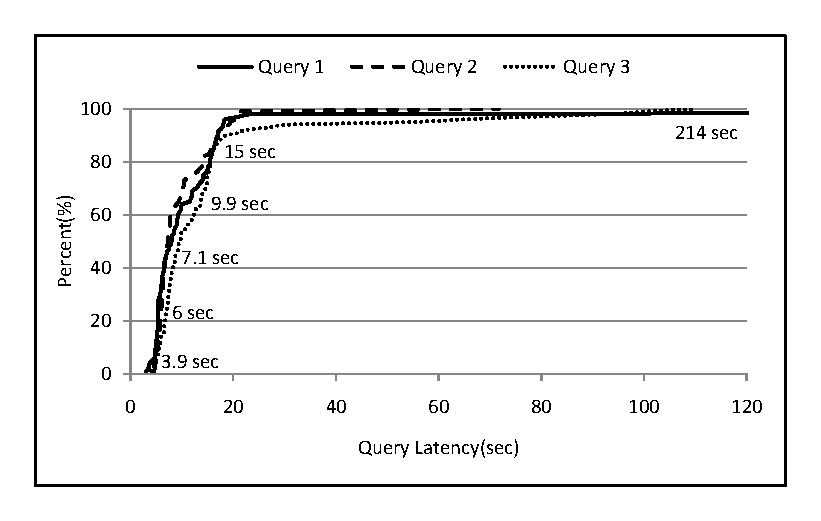
\epsfig{file=planet.eps, width=3.4in}
\caption{Cumulative distribution of query latency on the PlanetLab with about 600 nodes}
\end{figure}
\section{Related Work}
We have already discussed a range of related works which are closely tied to the MapReduce based query system in the previous sections. 
In this section, we will discuss some related works by dividing into three categories:
Range Query System On a P2P Network, Cluster Monitoring System, and Information Aggregation Algorithm.

\textbf{Range Query System on a P2P network}: Kim et. al\cite{can_query}, Squid\cite{squid}, and Artur et. al\cite{query_for_grid} discuss resource locating methods using a multiple dimensional P2P network. 
Kim et. al\cite{can_query} maps each resource attribute to one dimension in the CAN network. For matchmaking, the requirement conforming zone is created based on the criteria described in the query, 
and nodes inside the requirement satisfying region are candidate ones for the requirement.
Squid\cite{squid}, and Artur et. al\cite{query_for_grid} converts multiple dimension spaces into one dimensional ring space. Using the correlation between the multiple dimension and an attribute value, 
the resource matchmaking is performed. 
Above methods need a local node's information update to neighbor nodes, because they use the information in order to select the optimal requirement matching nodes.  
In addition, adding new resource attributes results in additional dimensions which bring the increased number of neighbor nodes and more management status.

Similar to our work, Kim et. al\cite{chord_matching} and Armada\cite{armada} use a tree-structure to check requirement matching. 
Kim et. al\cite{chord_matching} uses the Chord as an underlying P2P network, and the resource information propagation tree is
constructed based on the node id. Each node needs periodic resource information update to the parent node, which shares same drawbacks with the SWORD.
Armada\cite{armada} assigns an Object ID based on the attribute value, and a partition tree is constructed based on the proximity of the object ID. 
To locate nodes, only the desired region of Object ID needs to be scanned. However, this query system does not support arbitrary matching, such as regular expression match or partial string match.
Mercury\cite{mercury} and SWORD\cite{sword} use a DHT system for matchmaking. 
Because the DHT entry should be updated periodically, these methods incur lots of bandwidth consumption for resource information update.

\textbf{Cluster Monitoring System}: Blue Eyes\cite{blueeyes}, Ganglia\cite{ganglia}, and Supermon\cite{supermon} are hierarchically structured cluster monitoring systems. 
The Blue Eyes\cite{blueeyes} provides a reliable monitoring system by running multiple management servers, which are constructed as a self-organizing hierarchical tree using a management server list. 
For the high system availability, monitoring data is replicated into multiple backup servers, and this replication requires lots of bandwidth consumption and may cause data consistency problems.
The Ganglia\cite{ganglia} uses gmond and gmetad to aggregate local resource information. 
The Ganglia gmond gathers local cluster node's information using multicast, and the gmetad accumulates inter-cluster information by collecting the gmond information.
It also consumes lots of bandwidth for local node information update to the gmond, ann the system is not reliable in case of gmetad failure.
In the Supermon\cite{supermon}, the mon process is responsible for local resource information archiving and filtering, 
and the supermon process aggregates multiple mon processes' data and presents the aggregated data as a single data sample. 
The Supermon's hierarchical structure is not self-configurable, because the relation between mon server and supermon server has to be registered manually by a system administrator.
Intemon\cite{intemon} is a server-client model monitoring system. It uses the SNMP to collect resource information and supports automatic data analysis based on the historical resource correlation pattern.
Due to its static server-client relationship, it is not scalable in case multiple new clients join the monitoring system. The system also has to consume lots of bandwidth for periodical information update.

\textbf{Information Aggregation Algorithm}: 
Space Limitation. 
\section{Conclusions and Future Work}
This paper presents and evaluates the MapReduce based query system, which uses a self-organizing broadcast tree to spread queries to the entire network.
To our best knowledge, this system is the first real-world MapReduce application deployed on top of a P2P network.
We described how our system adapted the concept of Map and Reduce functional programming model and the differences between the Google MapReduce system and our MapReduce based query system.
With the aid of self-organizing boundedbroadcast method, we could distribute resource locating queries to the entire network neatly. 
The use of condor\_startd daemon to collect local resource information and ClassAd to process matchmaking allow us to perform various matching method(regular expression, partial string match) with plentiful resource information.
The analysis and simulation result show that dispersing query to the entire network with the novel boundedbroadcast method makes the queries to complete in a reasonable time, 
and they also show scability of our system for the increased number of nodes and resource attributes.
PlanetLab deployment of our system and its performance metric show that MapReduce based query system is a feasible and attractable solution for a wide area resource monitoring system.
Next steps for the MapReduce based query system are showing the practicability of a boundedbroadcast method on top of other P2P systems, such as Chord, Pastry, Can, and etc.
We will also work on deploying our MapReduce based query system in a real cluster for monitoring and querying purpose.
\bibliographystyle{abbrv}
\bibliography{hpdc_mr_ws}
\balancecolumns
\end{document}